\documentclass[12pt]{article}
%\usepackage{makeidx}
%\usepackage{multirow}
%\usepackage{multicol}
%\usepackage[dvipsnames,svgnames,table]{xcolor}
%\usepackage{graphicx}
%\usepackage{epstopdf}
%\usepackage{ulem}
%\usepackage{hyperref}
%\usepackage{amsmath}
%\usepackage{amssymb}

\usepackage[sorting=none]{biblatex}
\usepackage[french]{babel}
\usepackage[T1]{fontenc}
\usepackage{float}
\usepackage{graphicx}
\usepackage[utf8]{inputenc} 
\usepackage{csquotes}
\usepackage{pdfpages}
\usepackage{url}

\addbibresource{webographie.bib}

\title{Rapport de stage}
\usepackage[paperwidth=595pt,paperheight=841pt,top=56pt,right=56pt,bottom=56pt,left=56pt]{geometry}

\makeatletter
	\newenvironment{indentation}[3]%
	{\par\setlength{\parindent}{#3}
	\setlength{\leftmargin}{#1}       \setlength{\rightmargin}{#2}%
	\advance\linewidth -\leftmargin       \advance\linewidth -\rightmargin%
	\advance\@totalleftmargin\leftmargin  \@setpar{{\@@par}}%
	\parshape 1\@totalleftmargin \linewidth\ignorespaces}{\par}%
\makeatother 

% new LaTeX commands
\parindent=5pt

\begin{document}


\begin{center}

\vspace{3pt} \noindent
\begin{tabular}{p{439pt}}
\parbox{439pt}{\centering 
\includegraphics[width=125pt]{gallery/img-3.png}\textbf{{\large 

\includegraphics[width=146pt]{gallery/img-2.png}
}}
\includegraphics[width=132pt]{gallery/img-1.png}{\small  }} \\

$ $

\parbox{439pt}{\centering 
{\Huge Rapport de stage 2A}
} \\
\hline
\parbox{439pt}{\centering 
\textit{{\Huge Menou Camille}}
} \\
\parbox{439pt}{\centering } \\
\parbox{439pt}{\centering 
\textbf{\textit{{\Large Camille Menou}}}
} \\
\parbox{439pt}{\centering } \\
\end{tabular}
\vspace{2pt}

\end{center}



\begin{center}
\textbf{Ann\'{e}e 2016-2017}
\end{center}

\begin{center}
Stage de 2$^{e}$ année réalisé dans l'équipe \textit{COAST}
\end{center}

\begin{center}
\textit{Logo de l'entreprise}
\end{center}

{\raggedright
Maître de stage~: \textit{Philippe Kalitine}
\\
Encadrant universitaire~: \textit{Alexandre Parodi}\pagebreak{}
}

\begin{center}
\textbf{{\huge Déclaration sur l'honneur de non-plagiat}}
\end{center}

$ $

\textbf{Je soussignée,}

\textbf{Menou Camille}

\textbf{\'{E}lève-ingénieure régulièrement inscrite en 2$^{e}$
année à TELECOM Nancy}

\textbf{N$^\circ{}$ de carte d'étudiant(e)~:} 13538235

\textbf{Année universitaire~:} 2016 - 2017

\textbf{Auteur(e) du document, m\'{e}moire, rapport ou code informatique
intitul\'{e}~: Rapport de stage 2A}

$ $


Par la présente, je déclare m'être informée sur les
différentes formes de plagiat existantes et sur les techniques et normes de
citation et référence.

Je déclare en outre que le travail rendu est un travail original, issu de ma
réflexion personnelle, et qu'il a été rédigé entièrement
par mes soins. J'affirme n'avoir ni contrefait, ni falsifié, ni copié
tout ou partie de l'\oe{}uvre d'autrui, en particulier texte ou code
informatique, dans le but de me l'accaparer.

Je certifie donc que toutes formulations, idées, recherches, raisonnements,
analyses, programmes, schémas ou autre créations, figurant dans le
document et empruntés à un tiers, sont clairement signalés comme
tels, selon les usages en vigueur.

Je suis consciente que le fait de ne pas citer une source ou de ne pas la
citer clairement et complètement est constitutif de plagiat, que le plagiat est
considéré comme une faute grave au sein de l'Université, et qu'en cas
de manquement aux règles en la matière, j'encourrais des poursuites non
seulement devant la commission de discipline de l'établissement mais
également devant les tribunaux de la République Française.

\begin{center}
\textbf{Fait à Villers-lès-Nancy, le unjour/08/2017}
\end{center}

\begin{center}
\textbf{Signature~:}
\end{center}

\newpage

\newpage
\section*{Résumé :}

\section*{Abstract :}


%Pour insérer une image facilement :
%\begin{figure}[H]
%\centering
%\includegraphics[scale=0.4]{fichier de l'image}
%\caption[nom dans le sommaire]{légende}
%\label{fig:gallery}
%\end{figure}

\newpage
\section*{Sommaire}
\tableofcontents

\newpage
\setcounter{page}{1}
\addcontentsline{toc}{section}{Introduction}
\section*{Introduction}
Dans le cadre de ma deuxième année dans l'école d'ingénieur TELECOM Nancy, j'ai effectué un stage technicien au Laboratoire lorrain de recherche en informatique et ses applications (LORIA) \cite{loria} à Villers-lès-Nancy. Durant dix semaines j'ai travaillé au sein de l'équipe COAST \cite{coast} dirigée par François Charoy, du 6 juin au 11 août de l'année 2017. Ce stage m'a été proposé par Philippe Kalitine, ingénieur en recherche en informatique chez COAST.\\

L'équipe travaille actuellement sur MUTE \cite{mute}, un éditeur de texte collaboratif pair-à-pair open source (comprendre une application comme Google Doc mais sans avoir à stocker le document sur un serveur) qui a pour vocation de devenir l'éditeur de texte principal du personnel Inria \cite{inria}.\\

L'objectif de mon stage était de rendre l'éditeur riche, par exemple en intégrant des fonctionnalités autour de l'ajout de style dans les documents, d'images, de formules mathématiques, ou bien autour de l'exportation dans divers formats (PDF, HTML, etc.).\\

Dans le contexte de ce stage qui est celui de la recherche, il y a moins la pression d'une deadline, comme on le voit en entreprise. Cependant l'équipe COAST se prépare à faire une démonstration de MUTE lors de la quinzième European Conference on Computer-Supported Cooperative Work (ECSCW) \cite{ecscw} et qui aura lieu du 28 août au 1er septembre 2017 à Sheffield (UK). L'enjeu n'était donc pas moindre et suggérait un travail de qualité.

\newpage
\section{L'équipe COAST, INRIA : présentation}
\subsection{COAST}

\subsection{Moyens et stratégie}

\subsection{Organigramme du LORIA et de COAST}
Le LORIA est composé d'INRIA Nancy, du CNRS et de l'Université Lorraine.

\newpage
\section{Problématique du stage : rendre un éditeur de texte riche}
\subsection{Mise en contexte : MUTE}
MUTE est un éditeur web collaboratif temps-réel pair-à-pair. MUTE 

Oulala y'a des sous projets, entre autres Rich Text Editor.

\subsection{Description et analyse du problème posé : apporter une édition riche}


\subsection{Cahier des charges}
Le cahier des charges du projet Rich Text Editor a été défini comme étant les issues GitHub auxquelles j'ai été assignée. Les détails nécessaires m'ont été fournis à l'oral au moment opportun. Ci-dessous, la liste des issues que je devais réaliser pendant mon stage :\\

As a User I want to :
\begin{description}
    \item [see a partially styled (inline rendered style) Markdown text in the editor :]les balises doivent réapparaître lorsque l'utilisateur met le focus sur un élément contenant du style.
    \item [see a rendered version of my document :]cette issue est devenue obsolète du fait de la précédente (voir explications dans la partie Réalisation et validation). Concrètement, si l'issue précédente n'était pas réalisable immédiatement, MUTE aurait dû être divisée en deux parties : à gauche l'utilisateur écrirait le texte souhaité, à droite il aurait accès à un rendu où la syntaxe aurait été interprétée.
    \item [have an outline view for Markdown]
    \item [add basic styles (bold, italic...) to the document using keyboard shortcuts :]l'utilisateur doit pouvoir ajouter/enlever du style en utilisant des raccourcis claviers intuitifs, par exemple Ctrl+B pour le gras.
    \item [add basic styles (bold, italic...) to the document using toolbar :]au moment d'une sélection de texte, une barre d'outils doit apparaître pour que l'utilisateur puisse ajouter/enlever le style à la souris.
    \item [see my math formula rendered :]l'utilisateur doit pouvoir écrire une formule mathématique et qu'elle ait le même rendu que s'il l'avait écrite à la main.
    \item [include images into my documents :]tout est dans l'intitulé.
    \item [to add some "End of Page" character :]au bout d'un certain nombre de ligne, la page doit se terminer et une nouvelle doit être créée.
    \item [consult Markdown cheat-sheet :]l'utilisateur doit pouvoir rapidement accéder à la syntaxe de Markdown
    \item [consult MathJax cheat-sheet :]l'utilisateur doit pouvoir rapidement accéder à la syntaxte de MathJax
    \item [be able to export the document to another document format (PDF, plain text) :]tout est dans l'intitulé.\\
\end{description}

Les issues à propos des cheat-sheets et de l'exportation comportaient le tag "optionnal" pour dénoter une priorité basse. Les autres issues ont été classées par ordre de priorité décroissante, comme ci-dessus.

L'ensemble de mon travail était régi par un besoin fonctionnel incontournable : si des fonctionnalités visent à modifier le contenu du document alors le contenu doit effectivement être modifié, et ce pour n'importe quel collaborateur du document. Un autre besoin, non négligeable, était que les développements marchent à la fois sur Chrome et sur Firefox.

\newpage
\section{Réalisation et validation}
\subsection{Auto-formation}
Le stage a d'abord commencé par une période d'auto-formation à base de Massive Open Online Courses (MOOCs), de vidéos de conférences et d'articles écrits par des développeurs/ingénieurs de la communauté informatique. A cette occasion, et pendant les onze premiers jours je me suis donc formée en JavaScript et en TypeScript (JavaScript typé).\\
Le projet utilisant le framework AngularJS j'ai également lu à ce sujet grâce au apparemment assez célèbre Tour of Heroes \cite{tour}, projet Angular écrit pour un tutoriel disponible sur le site officiel d'Angular \cite{angular}.\\
De part le principe d'éditeur collaboratif, MUTE se sert de RxJS \cite{rxjs}, un ensemble de librairies visant à créer des applications JavaScript asynchrones et selon le paradigme de programmation événementielle.

\subsection{Environnement de travail}
La partie édition de MUTE est basée sur une API qui s'appelle CodeMirror \cite{codemirror}. Il s'agit d'un éditeur de texte écrit en JavaScript et pensé pour les navigateurs. Ce projet assez populaire (12,364 stars et 3000 forks au 4 août 2017) est agrémenté d'addons très utiles rendant CodeMirror très polyvalent.

L'ensemble du projet est hébergé sur un répertoire GitHub, un gestionnaire de version.

Il m'a été conseillé d'utiliser VisualStudio Code pour développer. Particulièrement adapté au langage JavaScript, VisualStudio permet de voir très facilement les fichiers modifiés par rapport au dernier commit et de faire des merges très simplement.

Le projet utilise le framework Angular.

Pour gérer ses dépendances, le projet utilise npm \cite{npm}, un package manager.

npm cz pour voir si le code est formaté correctement.

digest pour repérer des divergences.

\subsection{Méthode de travail}
Deux outils m'ont quotidiennement aidée à m'organiser et à prendre des notes pour faciliter l'écriture de ce rapport : l'outil de gestion de projet GitHub, ainsi qu'un journal quotidien que j'ai tenu selon le principe du bullet journal \cite{bullet}.

\paragraph{GitHub workboard}
Je le nomme workboard car il se présente comme un tableau référençant l'ensemble des issues m'étant attribués, de la documentation et ma roadmap. En voici un aperçu :

\newpage
\begin{figure}[H]
\centering
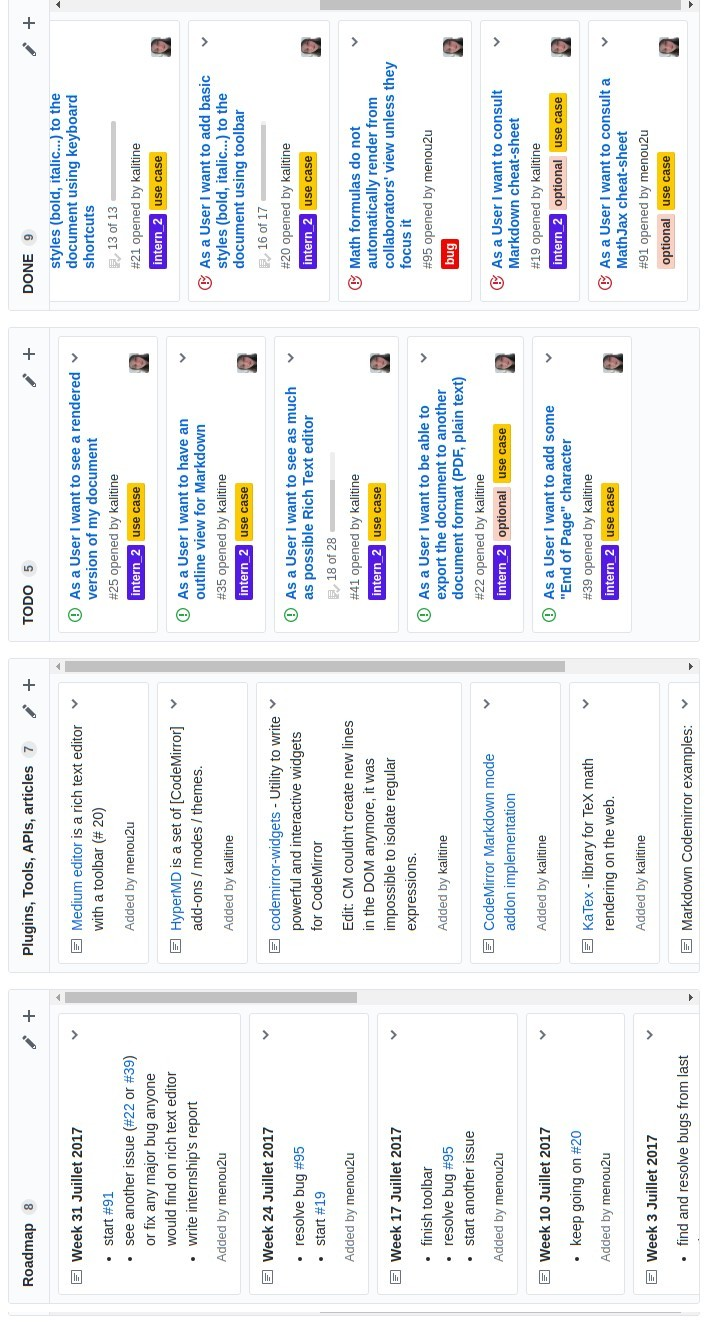
\includegraphics[scale=0.52]{gallery/workboard.jpg}
\caption[nom dans le sommaire]{Workboard du projet Rich Text Editor}
\label{fig:gallery1}
\end{figure}

\newpage
Tous les lundis matins je programmais ma roadmap. C'était également un excellent moyen pour accéder rapidement à mes issues et cela permettait également à mon maître de stage de pouvoir jeter un oeil à mon avancement. C'est une fonctionnalité de GitHub que je ne connaissais pas avant ce stage et qui se révèle être l'outil rêvé pour des fondus d'organisation.

\paragraph{Journal quotidien}
Afin de noter un maximum de choses pour écrire ce rapport mais aussi pour noter ma réflexion, ne pas oublier de faire quelque chose ou juste mieux m'organiser, j'ai pris l'initiative de tenir un journal quotidien de mon travail. A cette occasion j'ai repris quelques principes des bullet journals comme par exemple le fait de noter systématiquement les tâches à faire en organisant des checklists. Pour lier le workboard au journal, j'ai noté chaque jour sur quelle(s) issue(s) j'ai travaillé avec un code couleur pour retrouver plus rapidement des notes que j'aurais prises à l'intention de l'une d'elles.

\paragraph{Compléter une issue}
Avant de commencer une issue, j'en informais mon maître de stage qui me donnait certaines pistes de réflexion et de recherche à explorer avant de commencer.\\
Ainsi, en toute autonomie, je menais des recherches les plus exhaustives possibles pour trouver des solutions open source ou juste des méthodes que j'aurais pu reproduire dans notre projet. Nous voyions ensuite ensemble le meilleur choix.\\
Après le développement de la solution, je montrais le résultat, relevant les limites et recevant des détails à rajouter au développement.\\
Pour certaines issues, notamment pour les raccourcis clavier et la barre d'outils, je référençais sur l'issue correspondante l'ensemble des fonctionnalités présentes. Voici un exemple :

\newpage
\begin{figure}[H]
\centering
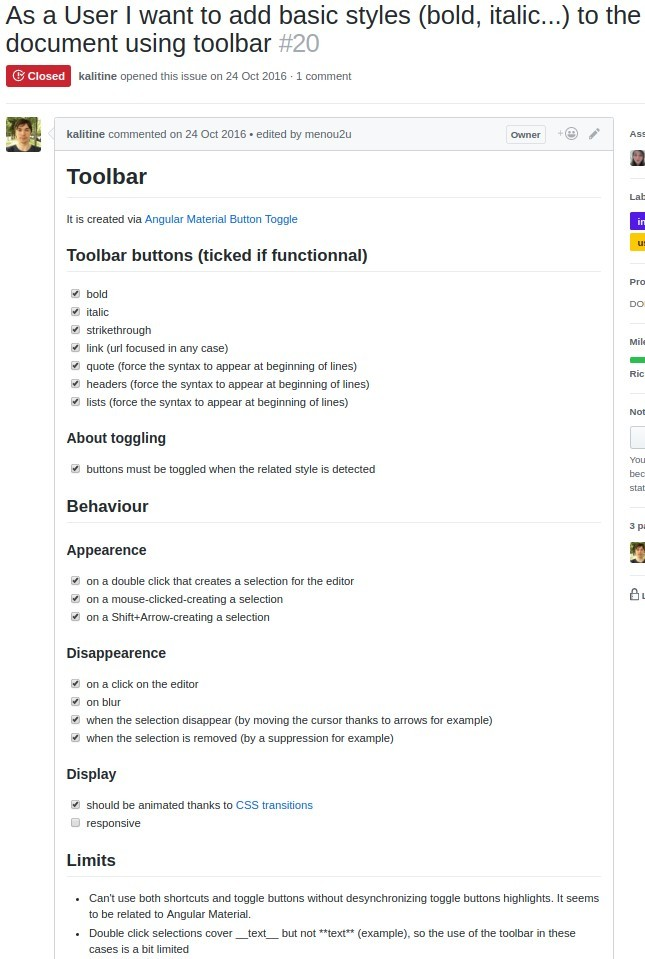
\includegraphics[scale=0.75]{gallery/issue.jpg}
\caption[nom dans le sommaire]{Issue associée à la barre d'outils}
\label{fig:gallery2}
\end{figure}

\newpage
L'avantage de cette pratique est qu'il sera possible pour les personnes qui maintiendront mon code de voir s'il y a eu des régressions ou tout simplement de voir ce qui existe déjà et ce qu'il reste à faire.

\paragraph{Communication avec l'équipe}
Lors des premières semaines, chaque vendredi 13h, l'équipe se réunissait pour faire état de l'avancement de chacun.
L'équipe utilise également Slack \cite{slack} pour communiquer.\\

\newpage
Abordons maintenant de manière plus concrète les différentes étapes de réalisation du cahier des charges.\\

\subsection{Cacher la syntaxe Markdown : intégration d'HyperMD}
Afin d'apporter du style à l'éditeur (gras, italique, etc.), l'équipe a décidé d'utiliser le langage à balise Markdown \cite{markdown}. A mon arrivée, MUTE était déjà configuré pour interpréter ce langage et l'on obtenait ce rendu :

\begin{figure}[H]
    \centering
    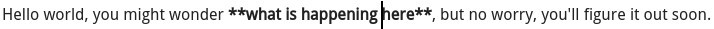
\includegraphics[scale=0.65]{gallery/style_example.jpg}
    \caption[nom dans le sommaire]{Syntaxe Markdown apparente}
    \label{fig:gallery3}
\end{figure}

L'on constate que le style est appliqué mais que les balises sont encore visibles. Comme indiqué dans le cahier des charges, l'une de mes tâches a été de faire en sorte de cacher la syntaxe.

\subsubsection{Une première approche à la main}
Il s'agissait de la première issue que j'avais à faire. Je n'avais pas encore à l'esprit l'importance de la contribution des gens dans le milieu open source. Car, encore une fois, CodeMirror est un projet assez populaire et le nombre de projets "dérivés" est important. Donc, dans un premier temps, j'ai essayé de résoudre le problème avec "les moyens du bord".\\
Dans mon analyse de la situation, j'ai remarqué que l'utilisation de la syntaxe Markdown au sein de l'éditeur modifiait le DOM \cite{dom}. Le DOM est une interface de programmation qui, entre autres, organise le contenu d'une page HTML en une structure d'arbre qu'il est possible de parcourir et modifier. Si on reprend l'exemple de l'image ci-dessus, on obtient le DOM suivant :
\begin{figure}[H]
    \centering
    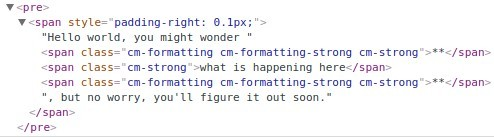
\includegraphics[scale=0.95]{gallery/modified_dom.jpg}
    \caption[nom dans le sommaire]{DOM modifié}
    \label{fig:gallery4}
\end{figure}
De ce fait, je pensais faire une recherche des noeuds du DOM dont les classes contiendraient des éléments en rapport avec le style CSS apporté par Markdown. Une fois ce style récupéré il aurait fallu l'appliquer uniquement au "what is happening here". Pour faire disparaître les balises sans pour autant les perdre, j'aurai essayé d'appliquer l'attribut CSS visibility en le met à "hidden" aux deux spans contenant les balises.
Cependant, cette solution paraissait trop lourde car elle nécessitait un parcours constant du document. De plus, si une personne avait été en train d'écrire, l'édition en aurait été gênée.

Mon maître de stage m'a alors suggéré de rechercher des API développées en ce sens à intégrer dans notre projet.

\subsubsection{Une première API : codemirror-widgets}
va falloir en parler viteuf\\
https://github.com/SamyPesse/codemirror-widgets


\subsubsection{HyperMD}
N'arrivant toujours pas à utiliser codemirror-widgets à nos fins, mon maître de stage m'a dirigée vers d'autres API, entre autres HyperMD \cite{hypermd}, projet datant de Janvier 2017, et dont la démo \cite{demo} paraissait remplir les objectifs de cette première issue et plus.
Après avoir installé HyperMD dans notre projet, nous avons constaté qu'en plus de cacher la syntaxe, les liens étaient stylisés, les images étaient prises en compte, ainsi que les formules mathématiques, grâce à MathJax \cite{mathjax}.\\


parler du service\\
faudra introduire un peu MathJax ici, comment ça marcher viteuf (back et front), dire qu'on a repéré un bug.\\
J'ai pris l'initiative de créer une issue pour créer une cheat-sheet pour MathJax, à l'instar de Markdown, afin d'améliorer l'expérience utilisateur.\\

\newpage
\subsection{Modifier le style}
\subsubsection{Ajout de raccourcis clavier}

\subsubsection{Création d'une barre d'outils}
parler de Material Angular, expliquer qu'un module c'est un Component Angular
parler des guidelines angular
parler de la désynchro
cacher sur téléphone

\newpage
\subsection{Adaptation des appels à MathJax}
\subsubsection{Analyse de la situation}
Lors de l'intégration d'HyperMD au projet, j'ai remarqué que si un collaborateur A décidait de modifier une formule, un collaborateur B ne verrait le changement que s'il mettait le focus sur cette formule. Même si cela ne reste qu'un bug d'affichage ne causant pas de divergences, j'ai proposé à mon maître de stage d'essayer de le corriger avant de m'occuper des cheat-sheets.\\
Dans un premier temps j'ai essayé de comprendre comment il était possible que le collaborateur B arrive à mettre à jour la formule. Il aurait été plus logique qu'au moment de focus ladite formule rien ne se passe de son côté, mais le fait est que si. J'en ai conclu que la syntaxe de la formule mise à jour était donc bien transmise aux collaborateurs.\\
J'ai pensé que l'information pouvait être stockée dans le DOM. Mais on constate (cf en Annexe) qu'aucune information n'est changée dans le DOM.\\
Pour mieux comprendre comment HyperMD fait appel à MathJax je suis allée voir le code source. Quand une expression du type "\$ ... \$" ou "\$\$ ... \$\$" est détectée, HyperMD créé une marque. Au sens de CodeMirror, une marque est ce qui est utilisé pour "marquer" une partie d'un texte en lui attribuant une classe CSS spécifique. Au moment de créer cette marque, il est possible de spécifier des options. Entre autres, HyperMD décide que l'élément DOM correspondant à cette zone de texte doit être remplacé par un élément span structuré comme suit :
span
    script\\
Or, grâce au script, MathJax est en mesure de générer un rendu, nommé dans la documentation MathJax "jax".\\
En consultant la documentation de CodeMirror, j'ai constaté qu'il était possible d'avoir accès à l'ensemble des marques. C'est dans cette liste que j'ai retrouvé la syntaxe de la nouvelle formule changée par A (cf Annexe). En mettant le focus sur la formule, le jax est retiré et la marqué est cassée : on retourne à un aspect d'édition de type "\$ ... \$". Or, comme la marque a été modifiée par A et transmise à B, le contenu de "\$ ... \$" affiché chez B sera bien ce qui se trouve chez A. Une fois que le focus est enlevé, la marque est recréée, MathJax est apppelé, et le jax est donc mis à jour. J'en conclus donc qu'il faut forcer MathJax à reprocéder au rendu des formules.\\

\subsubsection{Un premier fix}

\subsubsection{Doublons de marques : décalage des rendus}

\newpage
\subsection{Création d'antisèches}
Afin d'améliorer l'expérience des utilisateurs de MUTE, deux issues ont été créées pour ajouter des cheat-sheets à l'éditeur, littéralement des antisèches. Ces antisèches contiendraient des rappels de syntaxe pour Markdown et MathJax. Nous avons décidé avec mon maître de stage que ces éléments seront incrustés à droite du document, au même niveau que les informations le concernant (localisation du stockage et collaborateurs), afin que l'utilisateur puisse les avoir à portée tout en gardant accès à l'éditeur. Il m'a été suggéré de réfléchir à une solution à base d'onglets que je pourrais donc intégrer au niveau du composant nommé très justement "right-side".\\
Via mes recherches pour la barre d'outils, je me suis souvenue qu'Angular Material proposait un module Tabs (onglets) \cite{tabs}. J'ai donc immédiatement travaillé sur cette solution. J'avais alors deux manières d'organiser les informations : soit avoir trois onglets (Details, Markdown, MathJax), soit avoir deux onglets (Details, Cheat-sheets) avec dans Cheat-sheets deux onglets (Markdown et MathJax). J'ai opté pour la deuxième solution, car trois onglets prenaient trop de place, le nom des onglets était tronqué. De plus cela fait plus de sens de stocker toutes les cheat-sheets dans un même onglet.

\paragraph{Markdown Cheat-sheet}
Pour le contenu, et après avoir regardé des équivalents sur d'autres éditeurs, j'ai opté pour une disposition sur deux colonnes avec à gauche le rendu, à droite la syntaxe associée. L'idée que j'avais était d'avoir un rendu intuitif et raccord avec le reste de l'interface et les guidelines Angular.\\
J'ai tout d'abord essayé de travailler avec les tables HTML, mais le rendu était peu satisfaisant. Le fait de voir un tableau à cet endroit paraissait trop scolaire, le rendu était trop chargé.\\
Au hasard de mes essais, j'ai englobé le contenu dans un card, un autre composant Angular. Pour comprendre à quoi cela correspond, la zone d'édition du document, ressemblant beaucoup à feuille blanche, est un card. Le fait d'avoir fait ainsi m'a donné l'idée qu'il serait intéressant pour l'utilisateur de voir ce que le rendu donne sur le document. Ainsi, et pour donner de la structure à l'antisèche, j'ai mis le card en gris clair, puis y ait inséré six autres cards, eux en blanc. Chacun de ses cards représentera les catégories suivantes : les headers, les styles, les listes, les images, les liens et le code informatique. J'ai créé ces catégories en m'inspirant de cette cheat-sheet Markdown \cite{mdcheat}. Précédant chacun de ces cards, un titre en gris foncé, taille h2 permet de nommer chacune de ces catégories et sert de séparateur naturel entre chacun des cards.\\
Afin que les rendus soient fidèles à ce que génère HyperMD, j'ai eu l'idée d'importer la feuille CSS liée à HyperMD dans la feuille CSS du right-side. Ainsi, pour chaque texte auquel je voudrais appliquer le rendu HyperMD je n'aurai qu'à appeler la classe correspondante. Mais, pour certainement une bonne raison mais qui m'échappe, le style ne s'appliquait pas. Après plusieurs essais, j'ai décidé recréer des classes dans la feuille de style de right-side pour reproduire le rendu HyperMD.
Cette solution a marché mais cela a produit une duplication de code, il y a certainement moyen de faire autrement.\\
Après présentation à mon maître de stage, celui ci m'a suggéré que le fond gris clair soit de même couleur que l'arrière plan de l'application. Ainsi, les cards ressortent vraiment, sont à la même élévation que la zone d'édition et donnent un effet "post-it" qui est, je pense, vraiment parlant pour l'idée de mémo. L'utilisateur a donc une réelle idée du rendu que peut avoir ces différentes syntaxes.\\
Enfin, mon maître de stage a également suggéré que la cheat-sheet ait son propre composant Angular, sous-composant de right-side.

\paragraph{MathJax Cheat-sheet}
Pour cette antisèche, je suis partie sur le même concept d'apparence et de structuration.\\
Dans un premier temps, mon maître de stage et moi-même désirions que les rendus des formules soient générés par MathJax. MathJax étant utilisé uniquement par HyperMD, je n'avais jamais eu besoin de l'importer au sein de notre projet. Cette tâche seule s'est étalée sur trois jours. Pour ne pas pas perdre trop de temps, en parallèle, je commençais de mettre en place le composant qui allait contenir l'antisèche. Finalement, après que mon maître de stage soit venu m'aider à mettre en place MathJax, nous avons constater qu'une particularité de MathJax était bloquante : en effet, MathJax charge les formules globalement, sur l'ensemble de l'interface. Plus précisément : la liste de 'jax' mentionnée en 3.6 est unique à la page. Ainsi, les rendus se retrouvaient décalé : la première formule dans l'éditeur avait son rendu dans l'antisèche, et toutes les autres formules se trouvaient décalée de un cran.\\
Nous avons donc conclu qu'il serait plus simple que les rendus dans l'antisèche soient des images provenant d'impressions d'écrans. L'avantage à cela est que le rendu correspondra tout à fait à ce que MathJax produit dans l'éditeur, de plus, cela fait moins de formules à charger lors de l'affichage de l'antisèche.

\paragraph{Inconvénients}
HyperMD prévoit que tout texte collé dans l'éditeur à partir du presse-papier soit automatiquement échappé. Par exemple, *Hello world!* devient \textbackslash*Hello world!\textbackslash*. Il en va de même si l'utilisateur choisit de copier/coller la syntaxe d'un élément l'intéressant de l'antisèche vers l'éditeur. En soit ce n'est pas vraiment une mauvaise chose, car l'utilisateur pourra effectuer des manipulations avant d'enlever les caractères d'échappement et que le rendu ne se fasse. De plus les sections copiées ne sont pas très longues. Mais cela nécessite quand même une manipulation supplémentaire. Sans compter que pour des utilisateurs moins au fait de l'utilisation de l'éditeur cela peut poser un problème de compréhension.\\
Un autre inconvénient vient de l'utilisation des Tabs. Dans l'onglet Details se trouve l'affichage des contributeurs du projet. Il se trouve que le contenu de cet onglet refusait de prendre tout l'espace. Ainsi, le contenu était réduit à un très petit espace, qui, par conséquent, générait une barre de défilement, ce qui n'était pas très esthétique. Mon maître de stage a pris en charge la résolution de ce problème. Cela a eu un effet sur les antisèches, qui ne sont plus contenues dans un card gris, mais sont juste disposées sur le fond de l'application. Le résultat reste très sensiblement le même.\\
Le dernier inconvénient vient de la manière dont sont implémentées les Tabs d'Angular Materiel. La première fois que l'on décide de consulter les cheat-sheets, les deux sous-onglets se découvrent et l'on voit par défaut la cheat-sheet Markdown. Or, l'onglet Markdown n'est pas marqué comme étant sélectionné.\\

\begin{figure}[H]
    \centering
    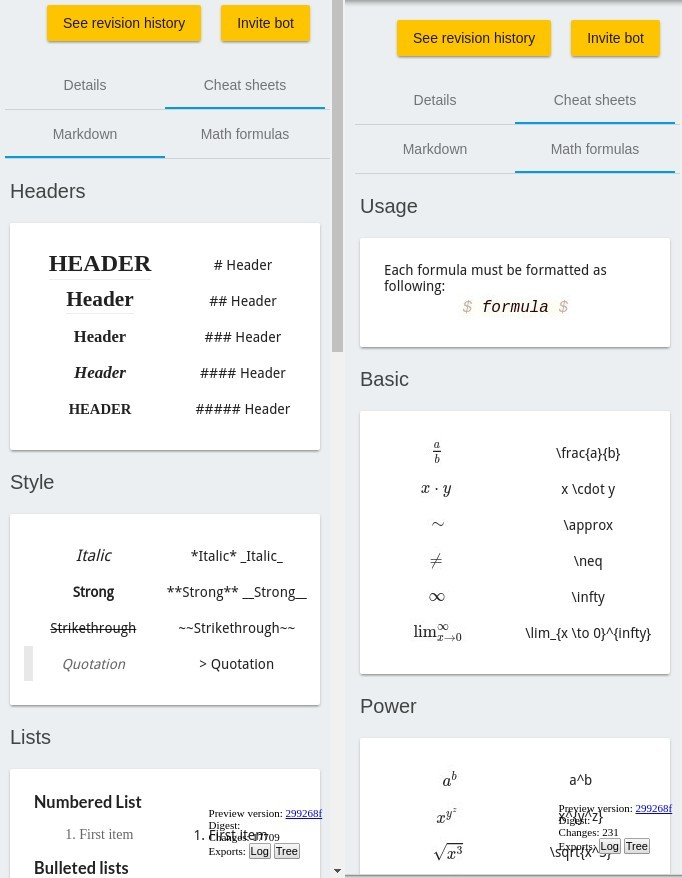
\includegraphics[scale=0.7]{gallery/cheat-sheets.jpg}
    \caption[nom dans le sommaire]{A gauche l'antisèche Markdown, à droite l'antisèche MathJax}
    \label{fig:gallery5}
\end{figure}


\newpage
\subsection{Tests}
Au cours du stage, il est arrivé que mon aide soit requise pour des tests. En effet, si l'on peut plus ou moins tester la robustesse de notre développement en ouvrant plusieurs navigateurs à la fois, il est impossible de reproduire l'édition simultanée d'un document par plusieurs collaborateurs. C'est pourquoi mon maître de stage, d'autres collègues, voire même moi-même demandions un coup de main à d'autres. Ces tests permettaient aussi que d'autres mettent en avant des scénarios où le développement de l'un ou de l'autre était incomplet.\\
De plus, avant que François Charoy décrète la fin du semestre et donc la fin des réunions hebdomadaires, chaque compte rendu de réunion était pris via MUTE. Nous pouvions ainsi tester la dernière démo, ce qui permettait de mettre en avant des oublis, des bugs ou des précisions sur les cas d'utilisations.\\

Digest ?

\newpage
\section{Bilan du stage}
\subsection{Avancement par rapport au cahier des charges prévu}
oulala j'ai tout fait à part EOP et exportation. J'aurai pu faire settings (refresh des formules, pop de la toolbar, animation des curseurs, preview MathJax) aussi.

\subsection{Retombées}

\subsection{Développement futur}
mathjax : compter les '\$'
settings

\subsection{Devenir de MUTE}

\newpage
\addcontentsline{toc}{section}{Conclusion}
\section*{Conclusion}

\newpage
\addcontentsline{toc}{section}{Remerciements}
\section*{Remerciements}
Mes tout premiers remerciements sont adressés à Philippe Kalitine, ingénieur de recherche chez COAST et mon maître de stage. Merci de m'avoir fait vivre ces dix semaines instructives tant au plan professionnel que personnel.\\

Merci à TELECOM Nancy pour la mise en place de cette période de stage afin que ses étudiants de seconde année puissent acquérir une expérience technique indispensable à la formation d'un ingénieur.\\

Merci à mon encadrant universitaire, Alexandre Parodi pour la supervision de ce stage et la lecture et notation de ce rapport.\\

Merci Laurent Bidet pour le deuxième écran, mine de rien ça change la vie !\\

De manière générale merci à toute l'équipe COAST pour sa convivialité. Venir travailler avec vous ce n'était plus du travail, mais l'exercice d'une passion commune dans une excellente ambiance !\\

Enfin surtout merci à toute personne ayant lu ce rapport de stage.

\newpage
\printbibliography[heading=bibintoc,title={Webographie}]

\newpage
\addcontentsline{toc}{section}{Glossaire}
\section*{Glossaire}

\clearpage

\newpage
\addcontentsline{toc}{section}{Annexes}
\section*{Annexes}

\newpage
\section*{Mots-clefs :}
\textbf{MUTE, collaborative-editing, rich-text-editor}

\end{document}